For all the problems dealt with in this report, the environment is represented as a two dimensional polygon with holes. However, we restrict ourselves to only deal with environments with orthogonal, i.e. only consisting of horizontal and vertical lines. With another algorithm for tesselating the environment the other algorithms could work for any polygonal environment.

In order to enhance the performance, we discretize our environment using a grid. Each cell is either \emph{occupied} if one of its corners lies into an obstacle or \emph{free}.
The environment is then tesselated into convex areas, we use rectangles, $C_{1\leq i \leq n}$ each satisfying the following criteria.

\begin{criteria}[of Visibility]
 \emph{For all point $P$ in the environment, if each corner of $C_i$ is visible, then $C_i$ is completely visible}. In practice, it means that checking if a area is completely visible from a given point can be done in only $4$ raycasts (because a rectangle has $4$ cornes).
\label{visibilityCriteria}
\end{criteria}

%The three problems we investigate involve finding interesting points on the map. We use the following terminology:
%\begin{description}
%	\item[Waypoints:] 
%	\item[Points of surveillance:] All the points from which a specific area is completely visible.
%\end{description}

\subsection{Convex tesselation}

In order to solve our three problems, we need a convex tesselation of our environment. The algorithm used to create the convex tesselation is based on the work from \cite{CoopMinTime}. Figure \ref{convexTesselation} shows the convex tesselation generated by the algorithm \ref{algoConvexTesselation}.

\begin{algorithm}
This algorithm describes how to create a convex tesselation of our environment. Since the obstacles are all orthogonal, we construct our convex tesselation as rectangles aligned with the polygons.
\begin{enumerate}
\item Based on the grid, make a discretization of the environment $G(A)$.
\item Find a yet uncovered cell, $p$.
\item Start growing a rectange $C_i$ from $p$ until its length and width reach $R$\footnote{R is the maximum convex size in width and/or length. This parameter is used to guarantee the visibily criteria \ref{visibilityCriteria}}.
\item While uncovered cells exists, goto 2.
\end{enumerate}
\label{algoConvexTesselation}
\end{algorithm}

\begin{figure}[h!t]
	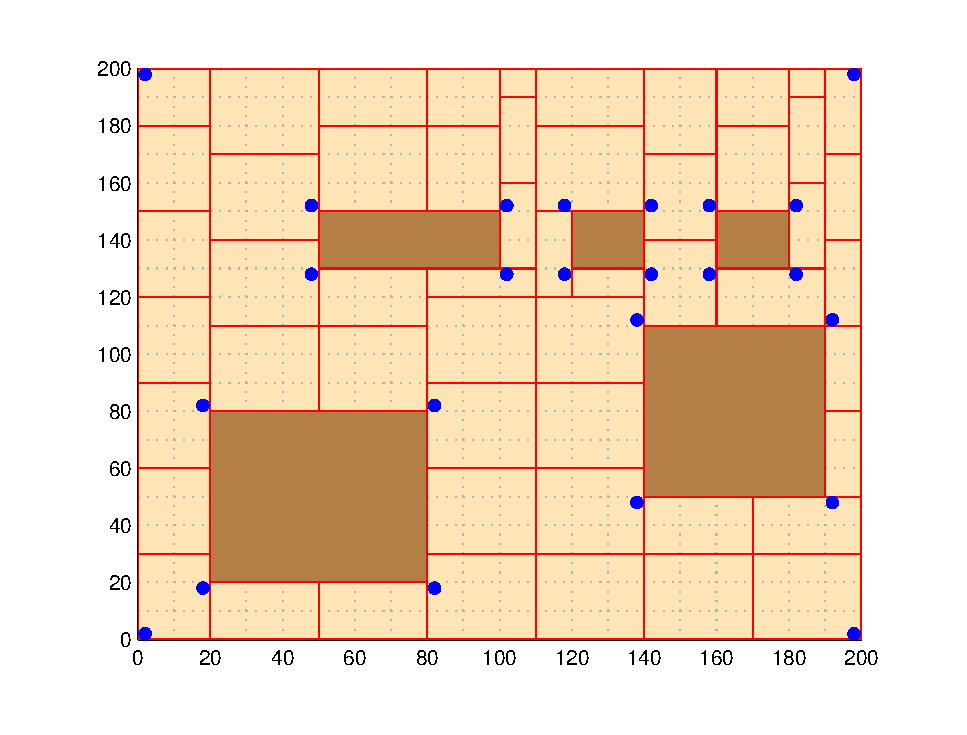
\includegraphics[width=\linewidth]{fig/convexCover.eps}
	\caption{Waypoints of the environment \& Convex tesselation ($R=3$)}
	\label{convexTesselation}
\end{figure}


\subsection{Graph representation \& search}
\begin{definition}[Waypoint]
Point at a given distance from an obstacle's corner (see Figure \ref{waypointNavigation}).
\end{definition}
For guard navigation in the environment, we perform an A*-search on the connectivity graph between the waypoints, also including the starting position and the goal position.
